\documentclass{article}
\usepackage{graphicx}

\title{ \textbf{Exploration of different Optimization Paradigms for the Sports Tournament Scheduling (STS) problem}}
\author{Matteo Preda - matteo.preda2@studio.unibo.it \\ Raffaele Sali - raffaele.sali@studio.unibo.it \\ Marco Zocco Ramazzo - marco.zoccoramazzo@studio.unibo.it}
\date{September 2025}

\begin{document}

\maketitle

\section{Introduction}
The report provides an in-depth study of the Sports Tournament Scheduling (STS) problem, emphasizing the formulation and comparison of different optimization models. The models examined in this project are built upon a shared formalization, which is outlined in the following section. The main goal of the presented work is to build a unified infrastructure for modeling, analyzing, and solving the STS problem, by considering the different techniques in these areas.  

\subsection{Model Formalization}

\paragraph{Input Parameters.}
The STS problem is defined by the following parameters, which are common to all models:
\begin{itemize}
    \item $n$: Number of teams (even number). Teams are indexed by $t \in \{1, 2, \ldots, n\}$ 
    \item $w = n-1$: Number of weeks. Weeks are indexed by $w \in \{1, 2, \ldots, n-1\}$
    \item $p = n/2$: Number of periods (matches per week). Periods are indexed by $p \in \{1, 2, \ldots, n/2\}$
\end{itemize}

\paragraph{Objective Variable and its Bounds.}
The objective function, which is only related to the optimization version, represents the maximum imbalance in home and away games for any team, with the goal of minimizing it:
\[
M = \max_{t \in \{1, \ldots, n\}} |h_t - a_t|
\]
where $h_t$ and $a_t$ represent the number of home and away games played by the team $t$, respectively. 
The theoretical upper bound for $M$ is $n-1$, while the lower bound for $M$ is $1$, since having an even $n$ implies that the matches each team plays (equal to $w$) are odd. For this reason, $h_t$ and $a_t$ must be different.

\paragraph{Constraints.}
All models rest on the following core constraints:
\begin{enumerate}
    \item Every team plays every other team only once in the tournament.
    \item Every team plays once a week.
    \item Each period in each week has exactly one game.
    \item Every team plays at most twice in the same period over the tournament.
    \item A team cannot play against itself.
\end{enumerate}

\paragraph{Pre-processing steps and Symmetry Breaking constraints.}
To increase solver performance, preprocessing steps might have been included in the examined models:
\begin{itemize}
    \item Building the model using a solver-independent language, like AMPL, which may require additional preprocessing time before the actual solving phase.
    \item Introducing implied constraints, such as the number of matches per team.
    \item Fixing the date of some matches to break team symmetries.
\end{itemize}

\subsection{Code Availability}
The project work can be found at \url{https://github.com/mpreda01/CDMO_project}.


\section{CP Model}

\subsection{Decision variables}

\subsection{Objective function}

\subsection{Constraints}

\subsection{Validation}

\section{SAT Model}

\subsection{Decision variables}

\subsection{Objective function}

\subsection{Constraints}

\subsection{Validation}

\section{SMT Model}

\subsection{Decision variables}

\subsection{Objective function}

\subsection{Constraints}

\subsection{Validation}

\section{MIP Model}

\subsection{Decision variables}

MIP model is based on binary decision variables that represent the occurrence of a match in a precise slot:

\begin{align}
x_{i,j,w,p} \in \{0,1\} \quad \forall i,j, w, p i \neq j
\end{align}

where $x_{i,j,w,p} = 1$ if team $i$ plays against team $j$ in week $w$, period $p$, with team $i$ playing at home and team $j$ playing away and $x_{i,j,w,p} = 0$ otherwise. The use of binary variables, instead of integer variables as in the CP model, has proven to be significantly less time consuming.

Furthermore, auxiliary variables are defined to facilitate the linear formulation of the objective function:
\begin{align}
h_t &\in \{0, 1, \ldots, n-1\} \quad \forall t \\
a_t &\in \{0, 1, \ldots, n-1\} \quad \forall t \\
M &\in \{0, 1, \ldots, n-1\}
\end{align}

where $h_t$ represents the number of games played at home by team $t$, while $a_t$ represents the number of games played away by team $t$, and $M$ represents the maximum home/away imbalance.


\subsection{Objective function}
Since the absolute value, used in the other optimization techniques, is a non-linear function, a different approach had to be used in order to produce a linear objective function. 
For this reason, the minimization has linked to two linearization constraints:

\begin{align}
& \text{minimize} \quad M \\
& h_t - a_t \leq M \quad \forall t \\
& a_t - h_t \leq M \quad \forall t
\end{align}

Thanks to these two constraints, it has been possible to represent the absolute value in a linear format, where the minimization leads $M$ to be equal to $\max_{t} |h_t - a_t|$.

\subsection{Constraints}

The model formalization described in section 1.1 has been followed in the MIP model too. All the constraints described below are linear.

\paragraph{General Constraints}

\begin{itemize}
    \item \textbf{Each slot has exactly one match:}
    \begin{equation}
        \sum_{i=1}^{n} \sum_{\substack{j=1 \\ j \neq i}}^{n} x_{i,j,w,p} = 1 \quad \forall w, p
    \end{equation}

    \item \textbf{Every team plays with every other team only once:}
    \begin{equation}
        \sum_{w=1}^{n-1} \sum_{p=1}^{n/2} (x_{w,p,i,j} + x_{w,p,j,i})  = 1 \quad \forall i,j, i < j
    \end{equation}

    \item \textbf{Every team plays once a week:}
    \begin{equation}
        \sum_{p=1}^{n/2} \sum_{\substack{j=1 \\ j \neq i}}^{n} (x_{t,j,w,p} + x_{j,t,w,p}) = 1 \quad \forall w, t
    \end{equation}

    \item \textbf{Every team plays at most twice in the same period over the tournament:}
    \begin{equation}
        \sum_{w=1}^{n-1} \sum_{\substack{j=1 \\ j \neq i}}^{n} (x_{t,j,w,p} + x_{j,t,w,p}) \leq 2 \quad \forall p, t
    \end{equation}

    \item \textbf{Given a time slot, at most one of the two possible home/away combination between each pair of teams may occur}
    \begin{equation}
        x_{i,j,w,p} + x_{j,i,w,p} \leq 1 \quad \forall w, p, i, j, i < j
    \end{equation}
\end{itemize}

\paragraph{Symmetry Breaking Constraints}

\begin{itemize}
    \item \textbf{Team symmetry:} Fix the schedule of the first week to break team symmetries:
    \begin{align}
        x_{2p-1,2p,1,p} &= 1 \quad \forall p \\
        x_{i,j,1,p} &= 0 \quad \forall p, (i,j) \neq (2p-1, 2p), i \neq j
    \end{align}

    \item \textbf{Team 1 opponent ordering constraint:}
It implies the matchups of team 1, by fixing that in week $w$, team 1 plays against team $w+1$:
\begin{equation}
    \sum_{p=1}^{n/2} \left( x_{1,w+1,w,p} + x_{w+1,1,w,p} \right) = 1 \quad \forall w
\end{equation}
\end{itemize}

\paragraph{Implied Constraints}
\begin{itemize}
    \item \textbf{Total matches per team:}
    \begin{equation}
        h_t + a_t = n - 1 \quad \forall t
    \end{equation}
\end{itemize}

\paragraph{Auxiliary Variable - Objective function}

The total number of games plays at home and plays away are defined using linear constraints:
\begin{align}
h_t &= \sum_{w=1}^{n-1} \sum_{p=1}^{n/2} \sum_{\substack{j=1 \\ j \neq i}}^{n} x_{t,j,w,p} \quad \forall t \\
a_t &= \sum_{w=1}^{n-1} \sum_{p=1}^{n/2} \sum_{\substack{j=1 \\ j \neq i}}^{n} x_{j,t,w,p} \quad \forall t
\end{align}

\subsection{Validation}
The MIP model was first built using AMPL, an algebraic modeling language for building and deploying optimization applications. AMPL has been chosen in order to exploit a solver-independent language which can be tested by multiple solvers without modifying the program design. In particular, four different solvers have been used:

\begin{itemize}
    \item CBC,
    \item HIGHS,
    \item CPLEX, 
    \item GUROBI.
\end{itemize}

The solvers have been applied to the model in Python, thanks to the package amplpy, which allows to work with .mod AMPL files in Python.

Solvers have been tested for the four different combinations of the two symmetry breaking constraints (both of them, none of them, only 1st team constraint or only 1st week constraint). Figure \ref{fig:MIP_dec} shows the solvers performance for the decision version, where each solver name is followed by:

\begin{itemize}
    \item \textbf{"None":} no symmetry breaking constraint has been used,
    \item \textbf{"st1":} only 1st team symmetry breaking constraint has been used,
    \item \textbf{"sw1":} only 1st week symmetry breaking constraint has been used, 
    \item \textbf{"st1+sw1":} both symmetry breaking constraints have been used.
\end{itemize}

\begin{figure}[H]
    \centering
    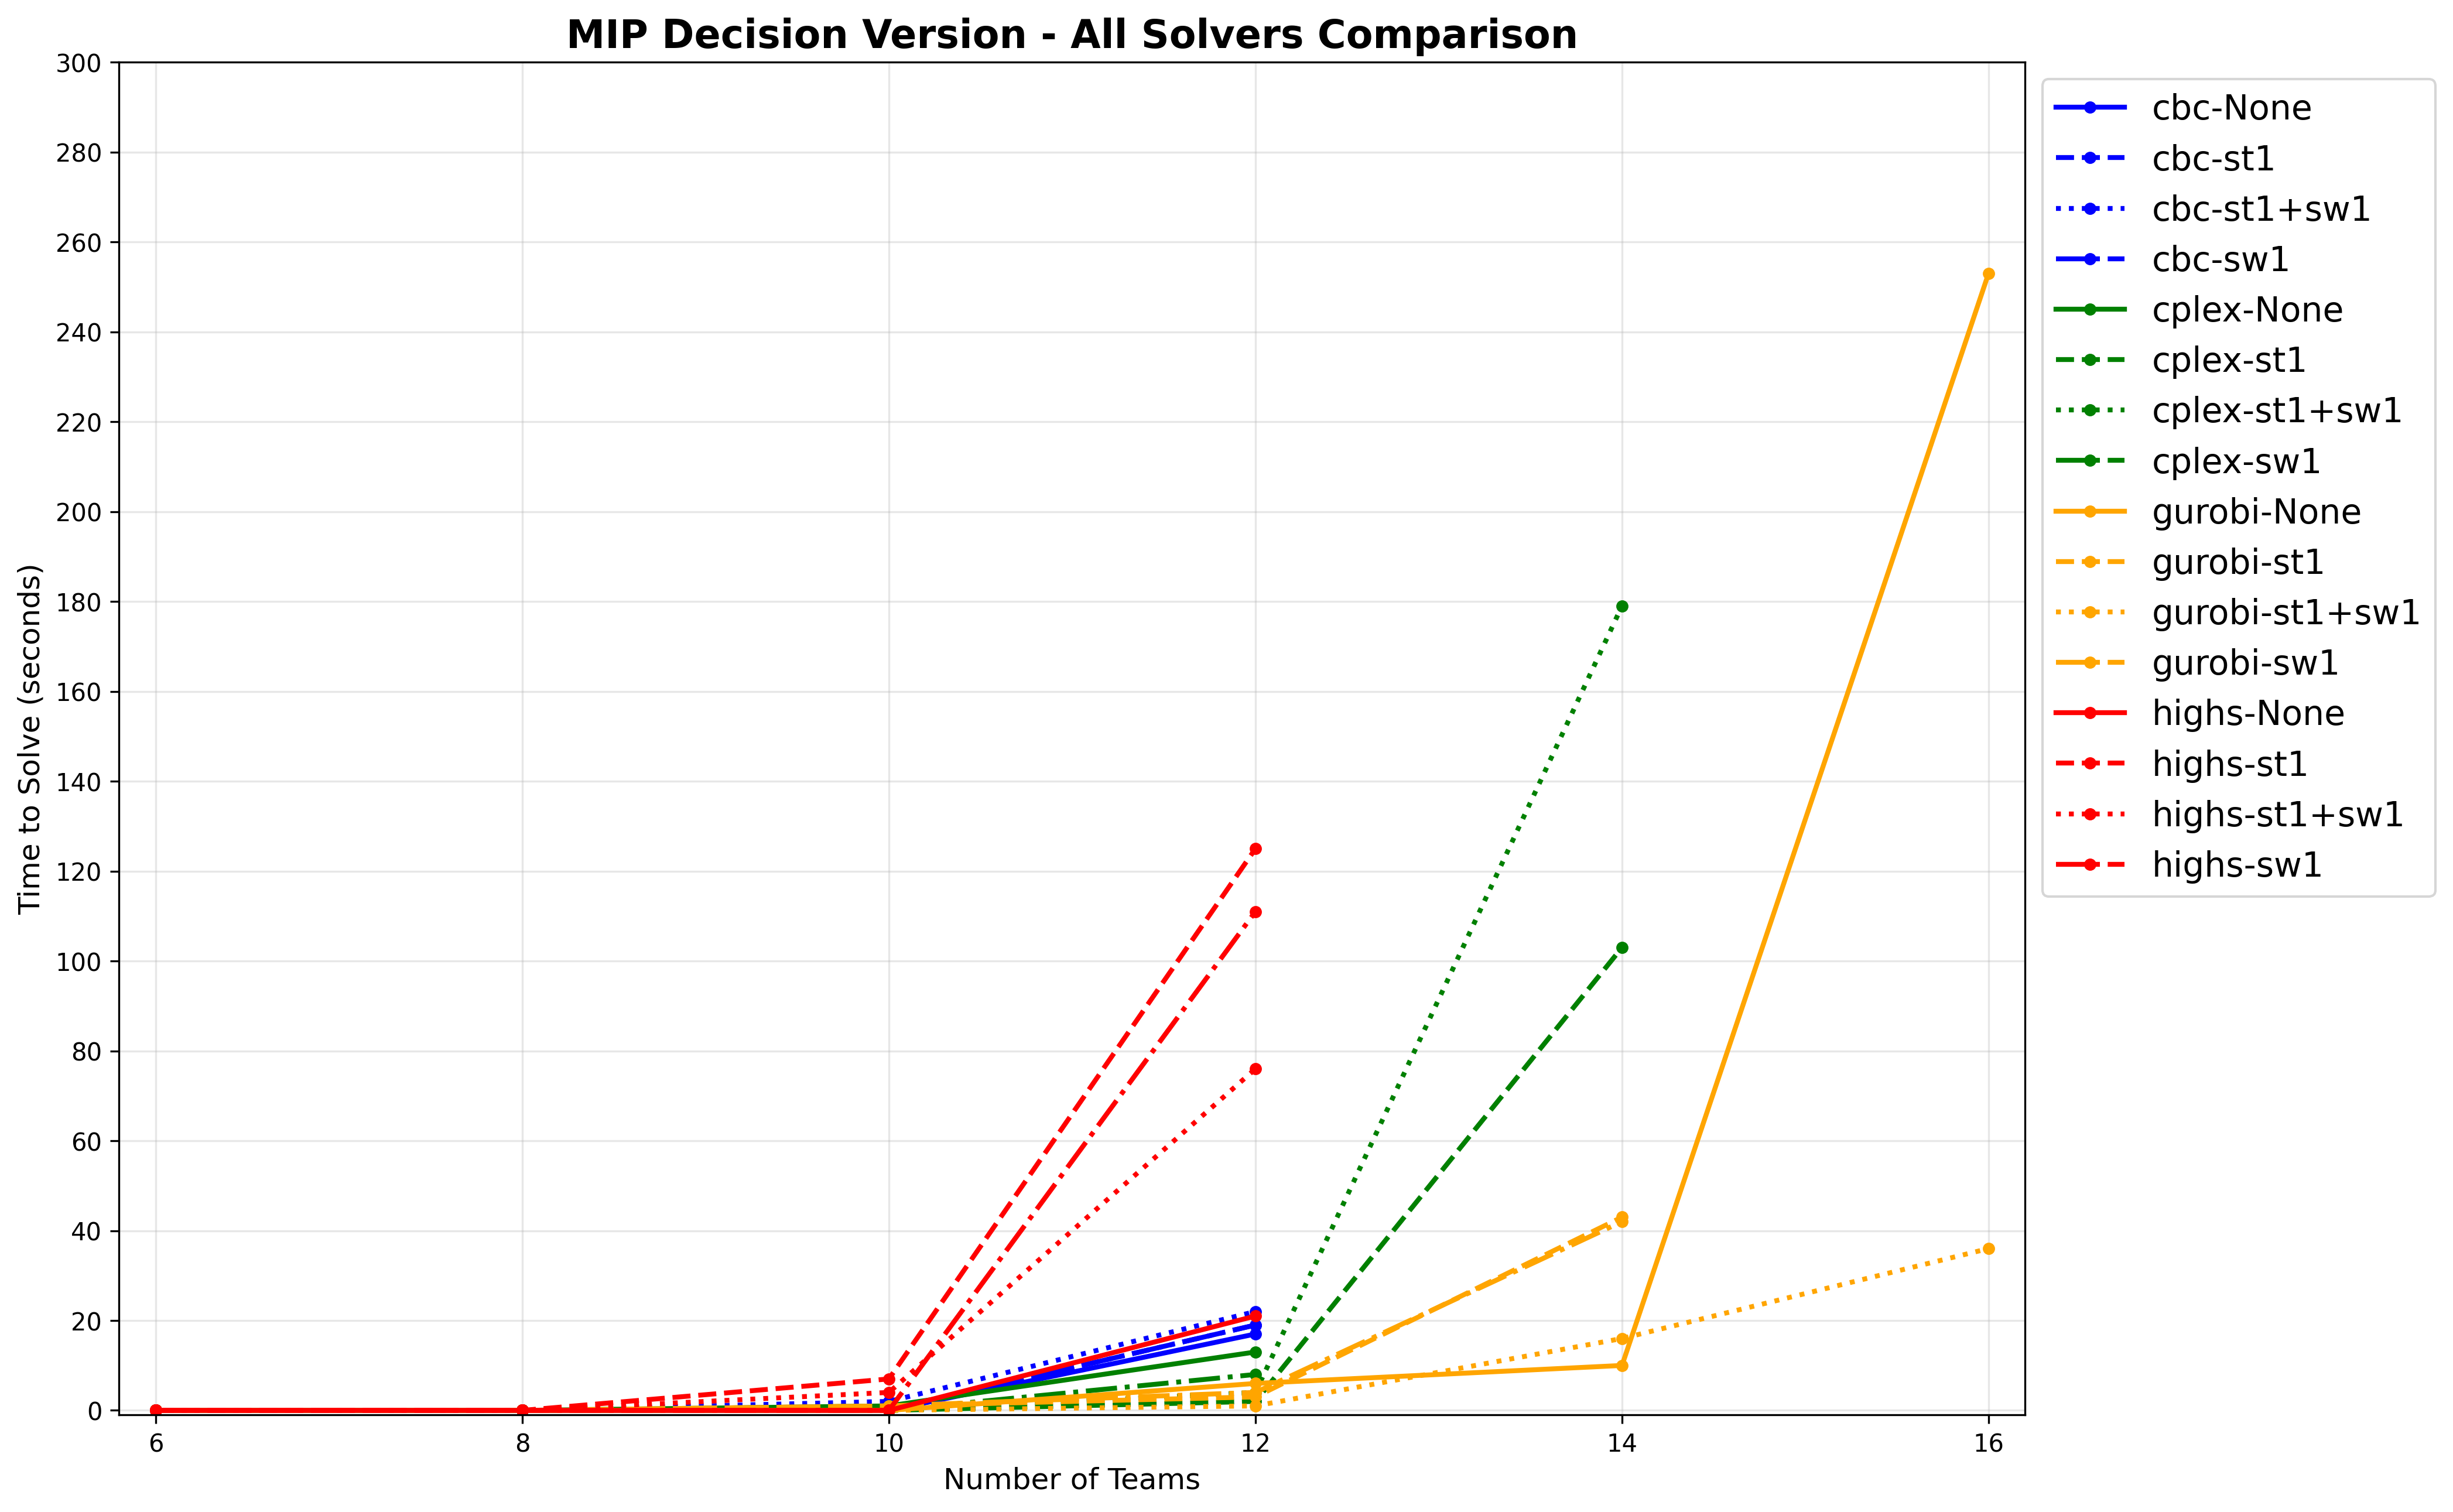
\includegraphics[width=0.7\textwidth]{../plots/MIP_decision.png}
    \caption{Solving time for different constraint configurations with MIP solver in decision version.}
    \label{fig:MIP_dec}
\end{figure}

Similarly, figure \ref{fig:MIP_opt} shows the performance in the optimization version.

\begin{figure}[H]
    \centering
    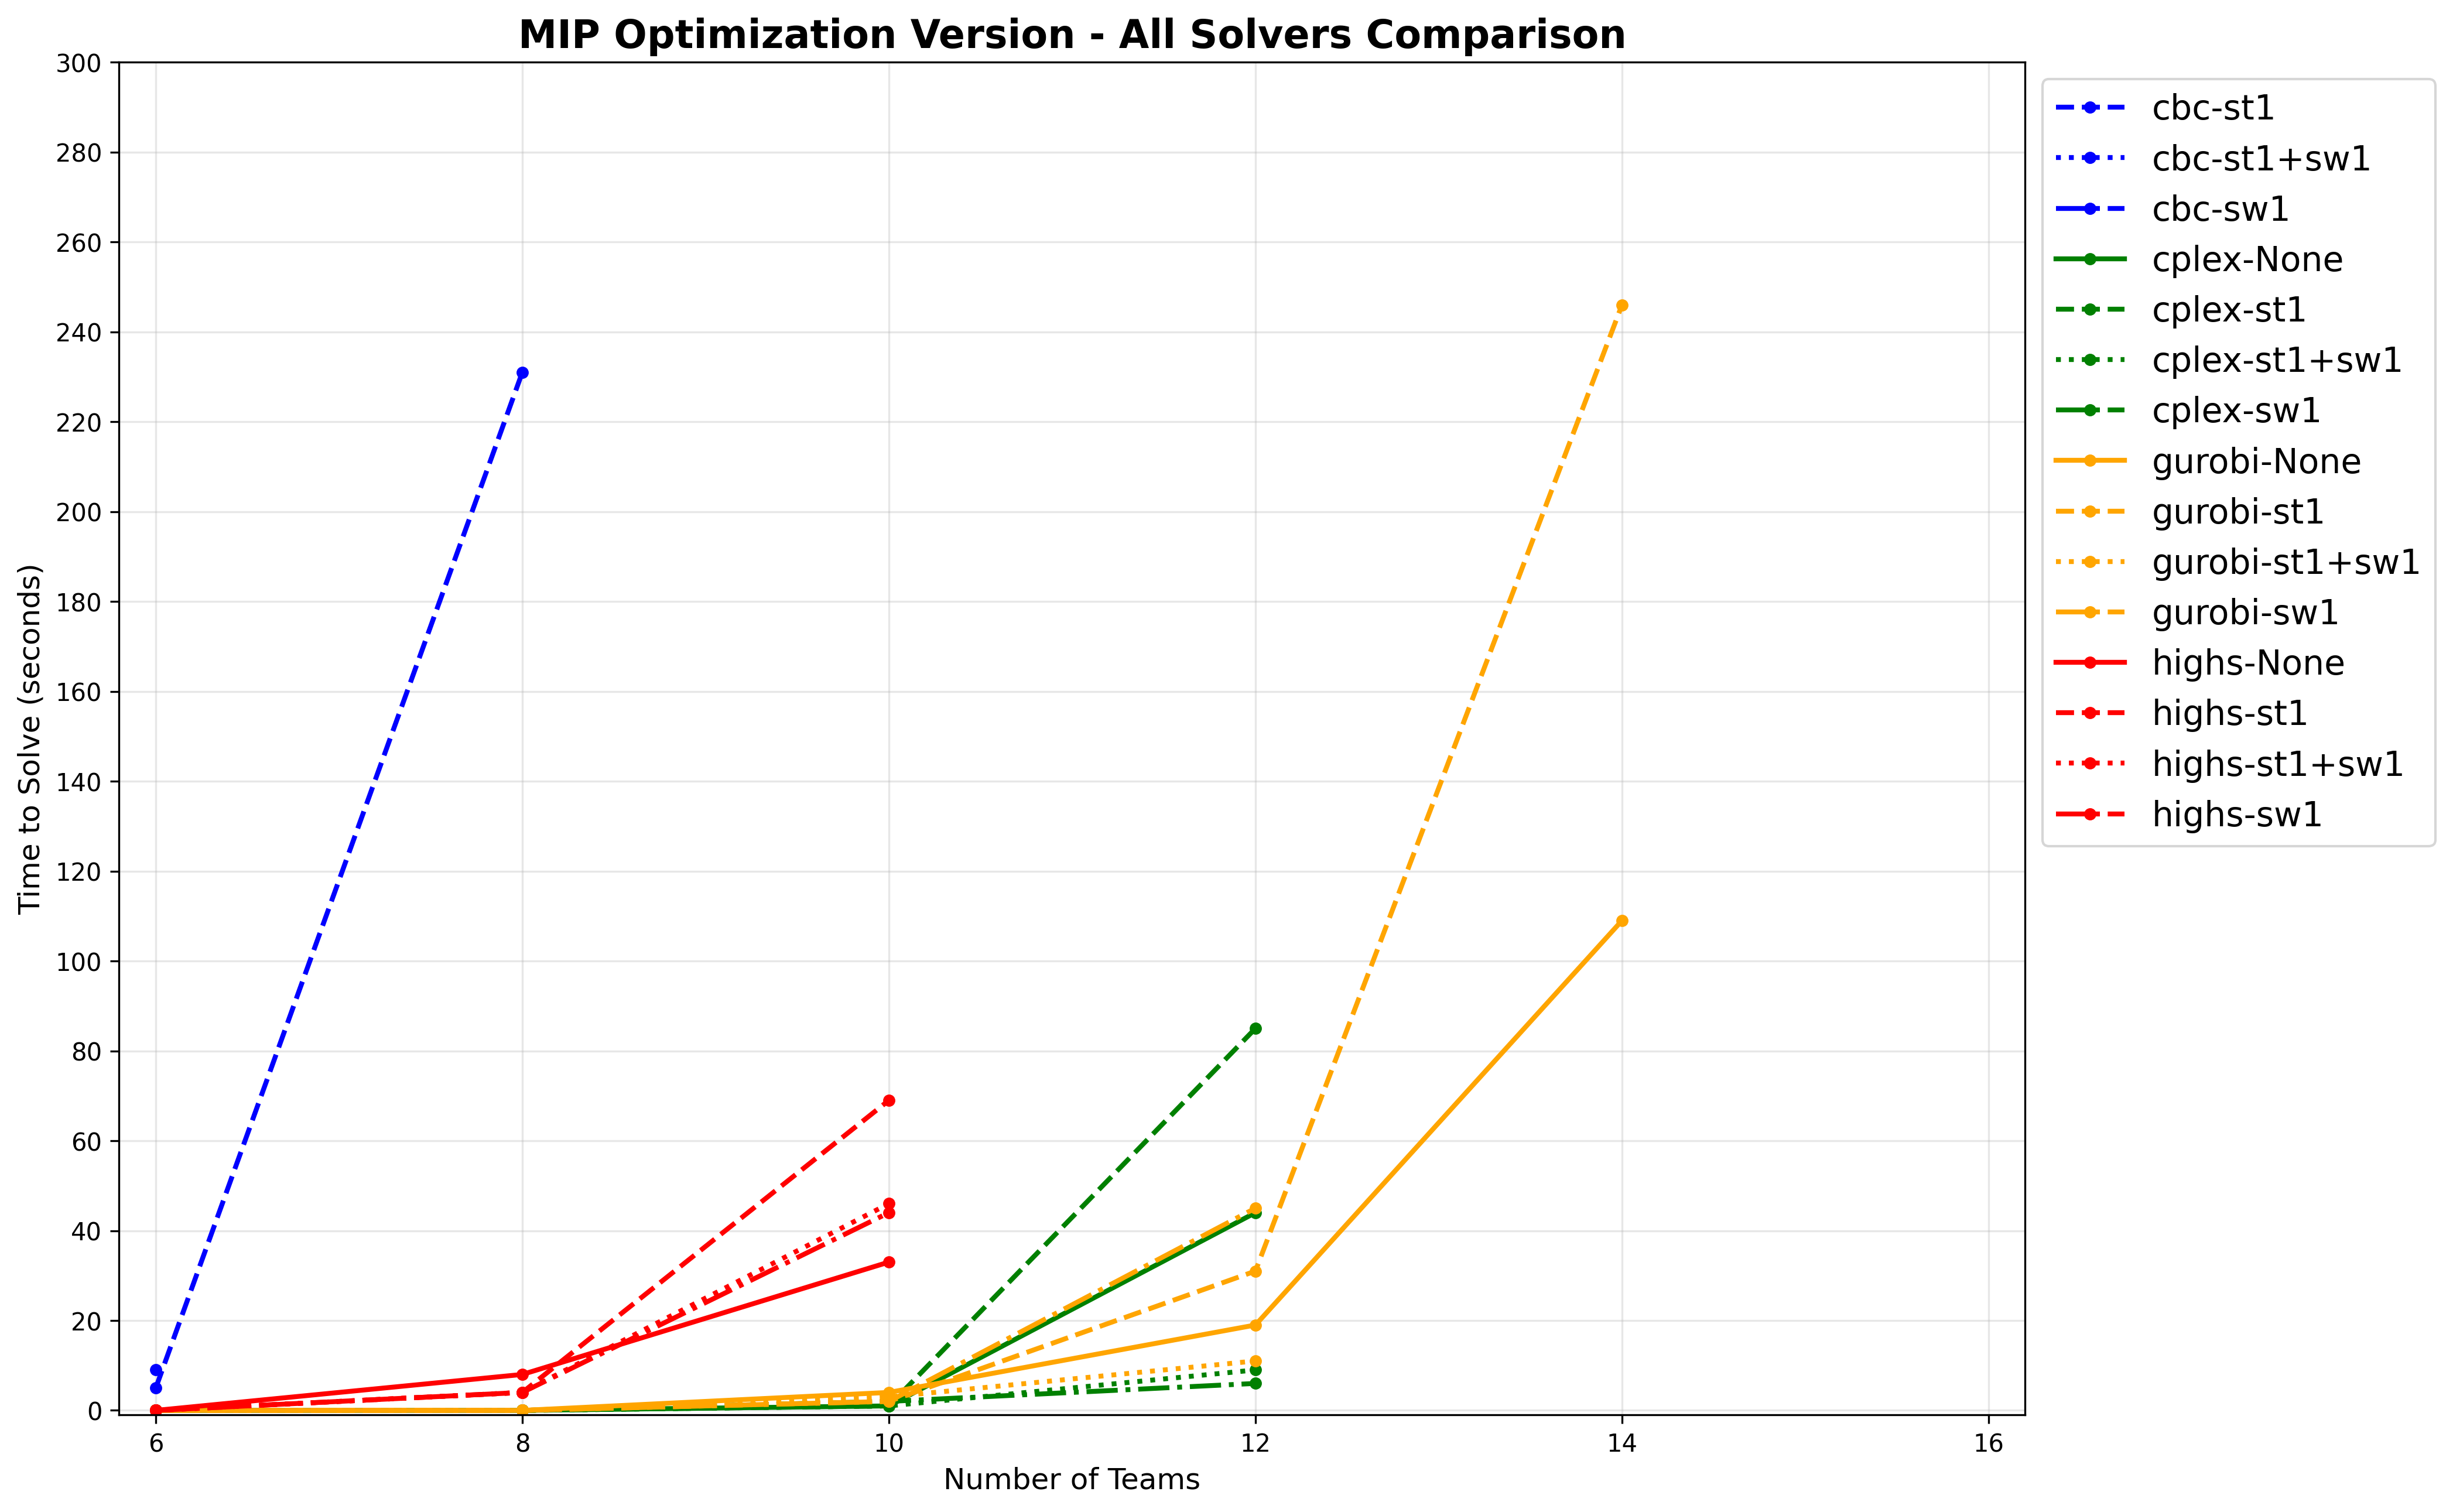
\includegraphics[width=0.7\textwidth]{../plots/MIP_optimization.png}
    \caption{Solving time for different constraint configurations with MIP solver in optimization version.}
    \label{fig:MIP_opt}
\end{figure}

\section{Conclusions}

\section{Authenticity and Author Contribution Statement}

\section{References}

\end{document}